\begin{refsection}
\chapter{Structures of closed and open states of the sodium channel Na\textsubscript{V}Ab}

The contents of this section were adapted from an article published in the \textit{Proceedings of the National Academy of Sciences of the United States of America}.\par
\bigskip
Reference: Lenaeus, M. J., Gamal El-Din, T.M., Ing C., Ramanadane, K., Pom\`es, R, Zheng, N., and Catterall, W. A. (2017) Structures of closed and open states of a voltage-gated sodium channel. \textit{Proceedings of the National Academy of Sciences of the United States of America}, 114(15), E3051-E3060.\par
\bigskip
Contributions: M.J.L., T.M.G., C.I., R.P., N.Z., and W.A.C. designed research; M.J.L., T.M.G., C.I., K.R., and R.P. performed research; C.I. performed all simulations; K.R. contributed new reagents/analytic tools; M.J.L., T.M.G., C.I., K.R., R.P., N.Z., and W.A.C. analyzed data; and M.J.L., T.M.G., C.I., K.R., R.P., N.Z., and W.A.C. wrote the paper.

\newpage

\section{Summary}

Bacterial voltage-gated sodium channels (BacNavs) serve as models of their vertebrate counterparts. BacNavs contain conserved voltage-sensing and pore-forming domains, but they are homotetramers of four identical subunits, rather than pseudotetramers of four homologous domains. Here, we present structures of two NaVAb mutants that capture tightly closed and open states at a resolution of 2.8-3.2 \AA. Introduction of two humanizing mutations in the S6 segment (NaVAb/FY: T206F and V213Y) generates a persistently closed form of the activation gate in which the intracellular ends of the four S6 segments are drawn tightly together to block ion permeation completely. This construct also revealed the complete structure of the four-helix bundle that forms the C-terminal domain. In contrast, truncation of the C-terminal 40 residues in NavAb/1-226 captures the activation gate in an open conformation, revealing the open state of a BacNav with intact voltage sensors. Comparing these structures illustrates the full range of motion of the activation gate, from closed with its orifice fully occluded to open with an orifice of $\sim$10 \AA. Molecular dynamics and free-energy simulations confirm designation of NaVAb/1-226 as an open state that allows permeation of hydrated Na$^+$, and these results also support a hydrophobic gating mechanism for control of ion permeation. These two structures allow completion of a closed-open-inactivated conformational cycle in a single voltage-gated sodium channel and give insight into the structural basis for state-dependent binding of sodium channel-blocking drugs.

\section{Introduction}

Voltage-gated sodium (Nav) channels are integral membrane proteins that change conformation in response to depolarization of the membrane potential, open a transmembrane pore, and conduct sodium ions inward to initiate and propagate action potentials \cite{Hille:2001tw}. As a result, sodium channels are paramount to nerve conduction, skeletal and cardiac muscle contraction, secretion, neurotransmission, and many other processes \cite{George:2005fm}. Nevertheless, the molecular mechanisms underlying voltage-sensing and sodium conduction remain uncertain due to the size and complexity of eukaryotic Nav channels, which are >200 kDa, contain 24 transmembrane segments, and remain resistant to detailed structural analysis \cite{Catterall:2000vb}.

Prokaryotic sodium channels (BacNavs), instead, have been used to study the 3D structure, mechanism of action, and pharmacology of Nav channels \cite{Ren:2001uo}. BacNavs contain the basic voltage-sensing and ion-conductance machinery of mammalian Nav channels in a much smaller package, typically consisting of homotetramers of subunits with 200-300 amino acids and six transmembrane segments, numbered S1-S6 by convention \cite{Ren:2001uo,Catterall:2015dh,Payandeh:2015hz}. NaChBac (from Bacillus haldorans) was the first BacNav to be cloned and studied by electrophysiology \cite{Ren:2001uo}, followed several years later by the purification, crystallization, and structure determination of its orthologs NavAb from Arcobacter butzleri \cite{Payandeh:2012ib,Payandeh:2013ex} and NavRh from Ricketsialles sp. \cite{Zhang:2013bz}, as well as pore-only constructs of NavMs from Magnetococcus marinus \cite{McCusker:2012di} and NaVAep1 from Alkalilimnicola ehrlichei \cite{Shaya:2014gg}. As predicted from structure-function studies of mammalian sodium channels, the S1-S4 segments form a voltage-sensing module in which four conserved arginine or lysine residues in the S4 segment serve as gating charges \cite{Bezanilla:2000gg,Catterall:2010kr}. The S5 and S6 segments form a pore domain similar to the ``inverted teepee'' of prokaryotic potassium channels, and the ion selectivity filter is formed by the P loop between them \cite{Catterall:2015dh}. The activation gate is located at the intracellular end of the S6 segments \cite{Catterall:2015dh}.

The voltage sensors of NaVAb and NaVRh are thought to be in an activated state, based on disulfide-locking and gating pore current studies \cite{DeCaen:2011ij,DeCaen:2009hc,DeCaen:2008eq,GamalElDin:2014bz}. BacNav crystal structures to date have shown a single activated conformation of the voltage sensor, but several different conformations of the pore domains, including the preopen state identified in the NaVAb/I217C structure and the collapsed potentially inactivated states identified in the NaVAb/WT and NaVRh structures \cite{Catterall:2015dh}. The intracellular activation gate formed by the bundle crossing of the S6 segments has been observed in different conformations in these BacNav structures, and several models have been proposed in which conformational changes in the voltage sensor are translated into pore opening by way of a concerted, iris-like dilation of the intracellular ends of the S5 and S6 segments, mediated by twisting and bending motions of the S6 helix \cite{Catterall:2015dh,Payandeh:2012ib,Bagneris:2014eh}. However, these models remain to be validated by structural comparisons of a single BacNav channel with intact voltage-sensing domains in both closed and open states. Here, we have used NavAb constructs to study the activation gate in two additional conformations, which allow accurate modeling of BacNav gating. Our results do not show any change in the structure of NavAb's voltage-sensing module, but they provide two crucial snapshots of the activation gate as it transitions from closed to open states and thereby allow comparison of the S6 helix in different states of the same channel. Molecular dynamics (MD) simulations confirm that the activation gate is open and suggest a hydrophobic gating mechanism for control of ion permeation.

\section{Results}

\subsection{NaVAb/1-226, a Mutant Captured in an Open State}
Trypsin digestion of NaVAb suggested a stable transmembrane core of the protein; therefore, we made a variety of C-terminal truncations to further study gating and improve crystallization. We found that NaVAb/1-226, which lacks 40 cytosolic residues of the CTD (Fig. \ref{fig:navofig2}), can be expressed at high levels and is suitable for studies by both electrophysiology and X-ray crystallography. This construct generated a Nav current with voltage dependence and kinetics of activation and inactivation during test pulses that were similar to those for NaVAb \cite{Lenaeus:2017bf}. However, there was an important distinguishing feature of the truncation mutant. NaVAb/1-226 activated at more negative voltages than full-length NaVAb, suggesting stabilization of the open state relative to the closed and inactivated states. In contrast, there was no change in the voltage dependence of steady-state inactivation of NaVAb/1-226.

These features suggested that the conformational state of NaVAb was perturbed by truncation of its CTD; a hypothesis we confirmed by X-ray crystallography. We crystallized NaVAb/1-226 containing the cysteine mutation I217C previously shown to facilitate crystallization in the full-length NaVAb channel. This mutant expressed well, could be purified easily, and could be analyzed by X-ray crystallography at high resolution (2.85 \AA). Like the NaVAb/FY structure, the NaVAb/1-226 structure showed near identity to the previously described structures in the voltage sensor and ion selectivity filter (RMSD of voltage-sensing module, 0.5 \AA; RMSF of selectivity filter, 0.25 \AA). Its activation gate, however, was significantly changed relative to previously described NaVAb and NaVAb/FY structures (Fig. \ref{fig:navofig6}), as highlighted by the blue arrows showing a diameter of 3.2 \AA \, for NaVAb/FY measured from the centers of nearest- approaching carbon atoms, compared with 10.3 \AA \, for NaVAb/1- 226. These changes in the diameter of the opening of the activation gate can be seen in more detail in spacefilling representations (Fig. {\ref{fig:navofig6} B). In NaVAb/FY, the side chains of I217 and M221 protrude into the lumen of the pore and fully occlude it, whereas the pore was open to the cytosol in NaVAb/1-226 (Fig. \ref{fig:navofig6} B).

The S6 helix is kinked in this structure compared with NaVAb/FY (Fig. \ref{fig:navofig7}, blue vs. tan). In addition, it has rotated away from the pore axis to increase the diameter of the permeation pathway to $\sim$ 10 \AA \, at the level of residue 217, sufficient to allow permeation of a hydrated sodium ion (see below). The kink at T206 corresponds to the hinge residue identified in structure-function experiments on prokaryotic sodium and potassium channels. On the intracellular end of S6, the conformation has clearly changed from the NaVAb/FY structure to the NaVAb/1-226 at the level of positions 217 and 221, resulting in a more open permeation pathway compared with all other NaVAb structures (Fig. \ref{fig:navofig7}). 

To illustrate the preferential movement of the activation gate in the NaVAb/1-226 structure, we plotted the pore diameters measured at the C$\alpha$ positions of the residues in the full S6 helix from extracellular vestibule (V) to intracellular activation gate (Fig. \ref{fig:navofig8} A). The pore diameters in NaVAb/FY (closed), NaVAb/ 1-226 (open), and NaVAb/WT (inactivated) are similar from the extracellular vestibule to the central cavity (CC), but differ strikingly at the activation gate which is closed in NaVAb/FY, wide open in NaVAb/1-226, and intermediate in NaVAb in the inactivated state. The changes in diameter of the activation gate at position 217, as observed from the intracellular side of the membrane, are illustrated in spacefilling format in Fig. \ref{fig:navofig8} C. These images confirm that NaVAb/FY is tightly closed, NaVAb/1-226 is open, and the slow-inactivated state observed for NaVAb/WT \cite{Payandeh:2013ex} is intermediate and asymmetric in shape. The CC (Fig. \ref{fig:navofig8} A), located in the lumen of the pore on the extracellular side of the activation gate, is a target site for binding of sodium channel-blocking drugs used in local anesthesia, cardiac arrhythmia, and epilepsy \cite{Payandeh:2012ib}. Even though the C? positions are not altered very much in transitions among these states, the twisting/bending motion of the S6 segment changes the positions of side chains NaVAb/1-226 compared with NaVAb/FY, as illustrated for T206 in Fig. \ref{fig:navofig8} B. The change in the conformation of this drug-receptor site indicates that transition from the open state to the deep resting state represented by NaVAb/FY is likely to have substantial effects on drug binding. A well-known feature of drug block of sodium channels is hyperpolarization-dependent drug dissociation, in which prolonged hyperpolarization reverses pre-established drug block \cite{Hille:1977td,Courtney:1975uu}. This rearrangement of the amino acid side chains involved in drug binding in the deep closed state represented by NaVAb/FY may contribute to this important aspect of state-dependent drug block and unblock.


\begin{figure}[!htb]
\centering
\includegraphics[width=0.5\textwidth]{navopen/NavOFig2}
\caption[The structure of NavAb/FY]{\textbf{The structure of NavAb/FY}. (\textbf{A})  The overall fold of NavAb/FY and a comparison with that of NavAb/I217C. One of four channel monomers is shown in either green or cyan to highlight the relationship between monomers. Lipid molecules are drawn in stick format. (\textbf{B}) NavAb/FY's closed activation gate and adjacent CTD. Amino acid residues lining the activation gate and neck are shown in stick representation (I217, M221, N225, and E228), as are lipids as in \textbf{A}. One subunit of the channel and its accompanying lipids have been removed for clarity.}
\label{fig:navofig2}
\end{figure}

\begin{figure}[!htb]
\centering
\includegraphics[width=0.5\textwidth]{navopen/NavOFig3}
\caption[Conformational changes at the activation gate]{\textbf{Conformational changes at the activation gate}. (\textbf{A}) Structures of NaVAb/FY and NaVAb/I217C are superposed in wire format. The view is as if one were below the channel and looking upward into the permeation pathway. Red arrows highlight the conformational changes described in the text; both an inward movement of the C-terminal portion of the S4-S5 linker and a rotation of the distal portion of the S6. (\textbf{B}) Close-up view of the interface between the S4-S5 linker and the S6 helix at the level of the activation gate. NaVAb/FY is on the left in gray, and NavAb/I217C is on the right in cyan. Helices are show in cartoon format; side chains as sticks; and atom distances are shown in red. (\textbf{C}) The view of the closed activation gate in NaVAb/FY (Left; gray) and NaVAb/ I217C (Right; cyan), with orientation as in A. Helices are shown in cartoon format, and side chains of I217 (for NaVAb/FY) and C217 (for NaVAb/I217C) are shown as yellow spheres.}
\label{fig:navofig3}
\end{figure}

\begin{figure}[!htb]
\centering
\includegraphics[width=0.5\textwidth]{navopen/NavOFig4}
\caption[The CTD of NavAb/FY]{\textbf{The CTD of NavAb/FY}. (\textbf{A}) Two of four NaVAb/FY monomers are shown as transparent surfaces, with underlying cartoons. Residues lining the CTD have been drawn in stick format, with hydrophilic residues highlighted in magenta and hydrophobic residues highlighted in orange. (\textbf{B}) Exemplar electron density of NaVAb/FY CTD neck, showing a ring of E228 hydrogen-bound to itself and an intersubunit hydrogen bond between E229 and H231. Helices are drawn in cartoon style, with side chains highlighted as sticks. Electron density is 2Fo-Fc calculated at 1.5 $\sigma$. (\textbf{C}) Exemplar electron density of NaVAb/FY CTD coiled-coil at the level of H239, highlighting the hydrophobic nature of the four-helix bundle at this level. Helices and side chains are displayed as described above. Electron density is 2Fo-Fc calculated at 1.5 $\sigma$, and chloride ion is shown as a green sphere. (\textbf{D}) Superposition of NaVAb/FY pore and neck (gray) and NaVAep1 pore and neck (light pink; PDB ID code 5hk7), with the voltage sensors and S4/S5 linkers of NaVAb/FY removed for clarity. (\textbf{E}) Superposition of NaVAb/FY coiled-coil (gray) with that of NavAep1.}
\label{fig:navofig4}
\end{figure}

\begin{figure}[!htb]
\centering
\includegraphics[width=0.5\textwidth]{navopen/NavOFig6}
\caption[Comparison of the activation gates of NavAb/ FY, NaVAb/I217C, and NavAb/1-226]{\textbf{Comparison of the activation gates of NavAb/ FY, NaVAb/I217C, and NavAb/1-226}. (\textbf{A}) The activation gates of NaVAb/FY (gray), NaVAb/I217C (cyan), and NavAb/1-226 (wheat) are indicated with blue arrows. Proteins are in ribbon representation, with two of four monomers and voltage sensors removed for clarity, and space filling representation of activation gate residues I217, M221 (above), and C217 (below). (\textbf{B}) Surface representation of NavAb/FY (gray), NaVAb/ I217C (cyan), and NaVAb/1-226 (tan), showing the difference in diameter across the activation gate (blue arrow). The activation gate measures 3.2 \AA across at M221 in the NaVAb/FY structure and 10.3 \AA across at C217 in the NaVAb/1-226 structure at the centers of the nearest C atoms.}
\label{fig:navofig6}
\end{figure}

\begin{figure}[!htb]
\centering
\includegraphics[width=0.4\textwidth]{navopen/NavOFig7}
\caption[Comparison of NavAb/FY, NaVAb/I217C, and NaVAb/1-226]{\textbf{Comparison of NavAb/FY, NaVAb/I217C, and NaVAb/1-226}. (\textbf{A}) Cartoon representation of the three structures of NaVAb shows the change in the position of S6 from as closed (NaVAb/FY), to preopen (NaVAb/I217C), to open (NaVAb/1-226) states. The view is from below the channel. A red arrow is shown to rep- resent the movement of the S6 helix as the channel moves through these states. (\textbf{B}) Side view of one pore module of each construct.}
\label{fig:navofig7}
\end{figure}

\begin{figure}[!htb]
\centering
\includegraphics[width=0.7\textwidth]{navopen/NavOFig8}
\caption[Comparing the diameter of the permeation pathway in closed, preopen, and open states of the pore]{\textbf{Comparing the diameter of the permeation pathway in closed, preopen, and open states of the pore}. (\textbf{A}) The pore diameter as measured by C$\alpha$ position (y axis) is shown as a function of position along the permeation pathway, including the external vestibule (V; residues 180-181), selectivity filter (SF) (residues 176-178), the CC-lining residues (CC; residues 206-210), and activation gate (residues 211-218) as discussed in the text. NavAb/FY is shown in gray, NavAb/1-226 is shown in wheat, and NavAb/WT is shown in green. (\textbf{B}) Close-up view of the CC of NavAb, highlighting the side chain of T206 and its conformational change as NavAb enters the preopen state. NavAb V213Y, a single mutant with similar properties to those of NavAb/FY, is shown in purple, and NavAb/I217C is shown in cyan. The NavAb V213Y structure was solved to 3 \AA resolution under nearly identical conditions and shows the same closed, activation gate conformation observed in NavAb/FY, though it was excluded from broad analysis here due to relatively poor electron density throughout the CTD. We use NavAb V213Y here to allow direct comparison of the position of T206 between closed and preopen states-such an analysis is impossible with our FY construct due to the phenylalanine mutation at position 206. (\textbf{C}) Close-up view of the activation gate at the level of residue 217. The view is as if one were below the channel and looking upward upon the permeation pathway. NavAb/FY is shown in gray, NavAb/1-226 is shown in wheat, and NavAb/WT is shown in green \textemdash with each model containing cartoon helices, transparent surface representation, and stick representation of the side chain at position 217.}
\label{fig:navofig8}
\end{figure}

\begin{figure}[!htb]
\centering
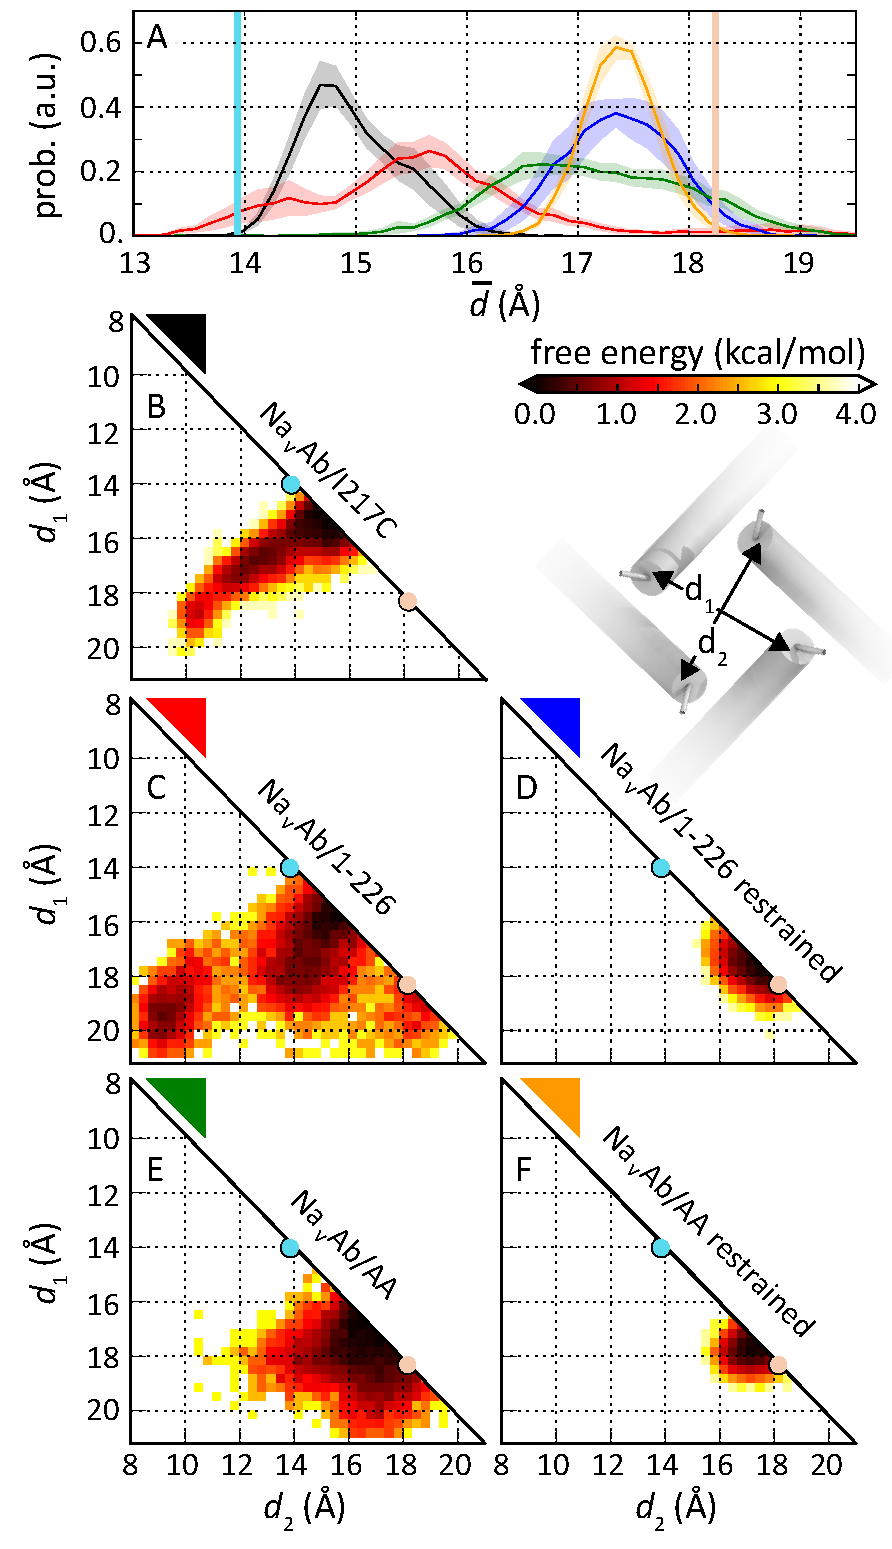
\includegraphics[width=0.5\textwidth]{navopen/NavOFig9}
\caption[Structural fluctuations of the activation gate]{\textbf{Structural fluctuations of the activation gate}. (\textbf{A}) Probability distribution of the mean diameters of the activation gate. NaVAb/I217C, black; NaVAb/1-226 restrained open, blue; NaVAb/1-226, unrestrained, red; NaVAb/AA restrained open, tan; NaVAb/AA unrestrained. a.u., arbitrary units; prob., probablility. (\textbf{B}) Free energy of the pairwise distances of residue 215-218 C$\alpha$ atom center of mass in diagonal subunits, d1 and d2, from molecular simulations with several channel models. (\textbf{B-F}) Free energy profiles are shown for: top row, NaVAb/I217C preopen state without TM restraints (black; \textbf{B}); middle row, NaVAb/1-226 without (red; \textbf{C}) and with (blue; \textbf{D}) TM restraints; and bottom row, NaVAb/V213A/C217A (NaVAb/AA) without (\textbf{E}) and with (\textbf{F}) TM restraints. The average pairwise distance of diagonal subunits in the open- and closed-state crystal structures are shown as pink and blue circles, respectively. Inset, a schematic representation of distances d1 and d2.}
\label{fig:navofig9}
\end{figure}

To examine the interplay of hydration, ion permeation, and structural fluctuations of the activation gate, we performed multiple MD simulations of NaVAb/I217C and NaVAb/1-226 in a hydrated lipid bilayer in the microsecond time range (Methods). Because the NaVAb/1-226 structure is a static snapshot of an apparently open conformation of the activation gate, we first examined results obtained by using harmonic restraints to keep the S6 helices close to the crystallographic structure of the open state. In these simulations, we observed a distribution of pore diameters at the centers of the S6 helices at the activation gate (Fig. \ref{fig:navofig9} A, blue), with a mean of $17.4 \pm 0.1$ \AA. In this restrained open state, there were relatively small fluctuations in the asymmetry of the S6 helices, as illustrated by the small deviations from the diagonal line in Fig. \ref{fig:navofig9} D. The mean hydration of the activation gate in this open-state structure was $15.1 \pm 0.8 $ water molecules (Fig. \ref{fig:navofig10} A, blue). Na$^+$ moved through this bottleneck with an average of $ 5.3 \pm 0.1$ water molecules in its inner hydration shell, compared with $5.8 \pm 0.1$ in free solution, indicating that passage through the open activation gate requires only the loss of $\sim$ 0.5 water molecule in the inner hydration shell of Na$^+$ (Fig. \ref{fig:navofig10} D). The estimated free energy barrier for Na$^+$ permeation was $\sim$2 kcal/mol (Fig. \ref{fig:navofig10} F), comparable with the free energy barrier for movement of Na$^+$ through the selectivity filter \cite{Chakrabarti:2013kd}. Together, these results are consistent with the conclusion that the NaVAb/1-226 structure captured by X-ray crystallography has an open activation gate, which presents no significant barrier to Na$^+$ permeation.

To study the effect of thermal fluctuations of the activation gate, we conducted similar simulations without restraints. In unrestrained simulations initiated in the NaVAb/1-226 or the NaVAb/I217C conformation, the activation gate spontaneously underwent moderate contraction and dilation, with changes in the average diagonal distances from the centers of the cylinders of the S6 $\alpha$ helices from $18.2 \rightarrow 15.7 \pm 0.2$\AA  and $13.9 \rightarrow 15.0 \pm 0.1$ \AA, respectively (Fig. \ref{fig:navofig9} A, black and red). Thermal fluctuations often led to significant deviations from the symmetric arrangement of the S6 helices, as shown by the deviations from the diagonal line in Fig. \ref{fig:navofig9} B (black and red). The activation gate bottleneck was completely dehydrated (dewetted) in the NaVAb/I217C preopen state (Fig. \ref{fig:navofig10} A-C, black), whereas it fluctuated between 0 and 25 water molecules, with an average of $7.3 \pm 0.4$, in unrestrained NaVAb/1-226 (Fig. \ref{fig:navofig10} A-C, blue).
To examine the effect of the hydrophobic side chains on the structure and properties of the activation gate, we replaced both C217 and V213 by alanine (NaVAb/AA) and repeated the simulations successively with and without restraints on helix position. In the restrained simulations, this double mutation resulted in a shift of helix geometry toward the open state relative to WT ($17.5 \pm 0.1$ vs. $15.7 \pm 0.2 $ \AA; Fig. \ref{fig:navofig9} A, D, and E) and greater hydration (Fig. \ref{fig:navofig10} A-C). Because of the smaller side chains, average pore hydration in NaVAb/AA was greater than in NaVAb/I217C in both unrestrained and restrained simulations ($20.5 \pm 0.6$ and $21.3 \pm 0.2$ water molecules, respectively). As such, Na$^+$ hydration in the activation gate only dropped to $5.5 \pm 0.1$ in the double mutant (Fig. \ref{fig:navofig10} D). However, this additional hydration had no effect on the free energy barrier for Na$^+$ movement, which was indistinguishable from that obtained from restrained simulations of the open NaVAb/I217C channel (Fig. \ref{fig:navofig10} F).

Together, the MD simulation results confirmed that the crystallographic structure of NaVAb/1-226 corresponds to an open state of the NaVAb pore, for which the activation gate induces a small desolvation penalty of $\approx$2 kcal/mol relative to the aqueous state. Structural relaxation led to a partial collapse and partial dehydration of the activation gate, which resulted in doubling the height of the Na$^+$ desolvation barrier to 4 kcal/mol, and to asymmetric fluctuations of the activation gate that were also observed in the closed state of the channel. These effects all but disappeared in the NaVAb/AA double mutant of the S6 helix, which remained close to the crystallographic structure of the open state, even in the absence of helix restraints. These results support a hydrophobic-collapse model for closure of the activation gate.

\begin{figure}[hp]
\centering
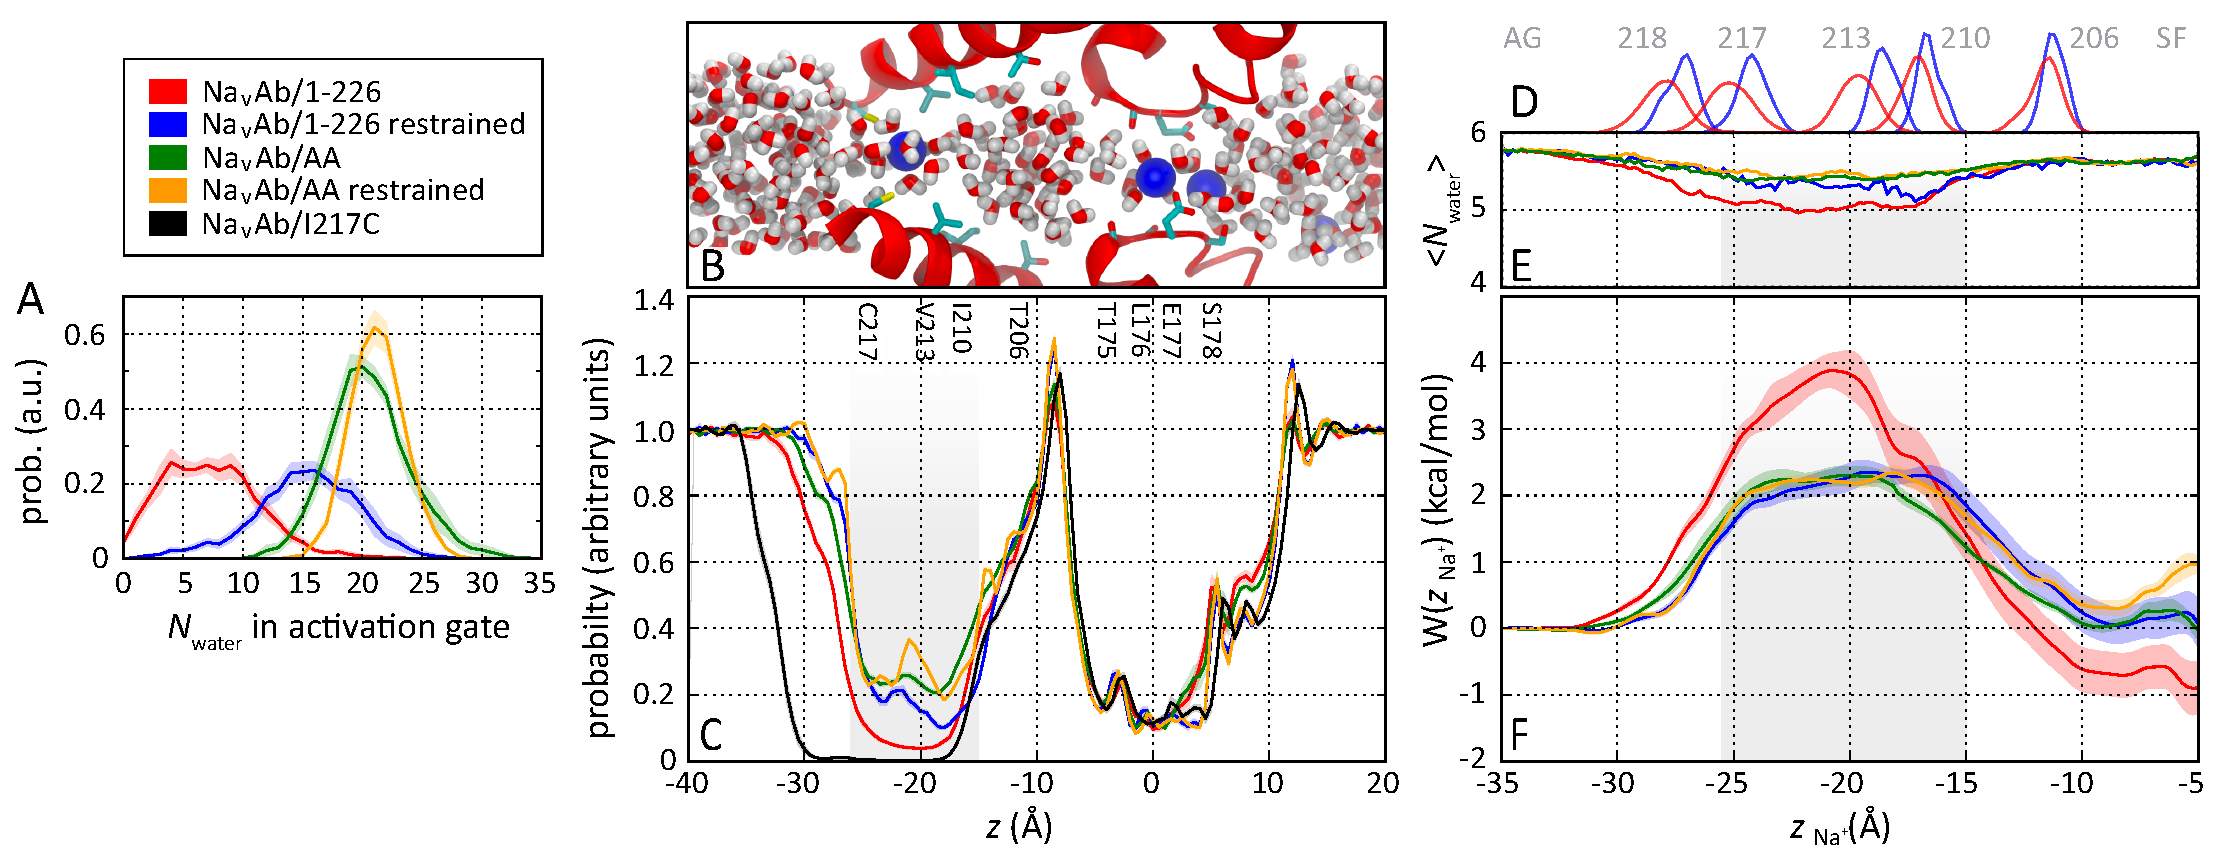
\includegraphics[width=0.9\textwidth]{navopen/NavOFig10}
\caption[Hydration and free energy of Na$^+$ conduction through the activation gate]{\textbf{Hydration and free energy of Na$^+$ conduction through the activation gate}. (\textbf{A}) Distribution of the number of water molecules, $N_{water}$, in the activation gate. Color coding is indicated in the key. (\textbf{B}) Snapshot of the unconstrained NaVAb/1-226 I217C channel with one Na$^+$ cation in the activation gate and two Na$^+$ cations in the selectivity filter shown as blue spheres. Two pore domain monomers are shown as red ribbons with selected side chains indicated below. Water molecules are shown as red and white licorice. (\textbf{C}) Distribution of water molecules along the pore axis. Scale and alignment are identical to \textbf{B}. The activation gate is highlighted in gray shading. (\textbf{D}) Axial distribution of C-alpha atoms of selected side chains lining the activation gate and the CC of the channel from restrained (blue) and unrestrained (red) simulations of NaVAb/1-226 I217C. AG, activation gate; SF, selectivity filter. (\textbf{E}) Average number of water molecules in the first hydration shell of Na$^+$ from bulk water (left) to the CC (right). (\textbf{F}) PMF profiles W($z_{Na^{+}}$) for movement of a Na$^+$ ion along the pore axis. Differences in the free energy of Na$^+$ in the CC (z > $\sim$15 \AA) are due to fluctuations in the number of cations present in the selectivity filter. In \textbf{C}, \textbf{E}, and \textbf{F}, the 11 \AA-wide barrier region is highlighted in gray shading. Data for NaVAb/I217C are only shown in \textbf{C} because the long, narrow dehydrated intracellular activation gate and the passage of Na$^+$ ions.}
\label{fig:navofig10}
\end{figure}

\section{Discussion} 

\subsection{S6 Mutations Reveal the Structure of NaVAb's Intracellular CTD}
Our FY structure revealed the conformation of the CTD of NaVAb in a closed state of the pore. It is a four-helix bundle similar to that observed in other BacNav channels and prokaryotic K$^+$ channels, as well as the pore-only construct of NaVAep1 and a NaK chimera \cite{Irie:2012dn,Arrigoni:2016fs}. In the highest-resolution structure of NaVAep1 (2.95 \AA), the portion of the CTD nearest to the pore contained a pi-helix that accommodated a centrally oriented tryptophan residue coordinating a chloride ion in the middle of the four-helix bundle. The NaVAb structure lacks this feature. Instead, there is a continuous alpha helix with two centrally oriented rings of polar residues (N225 and E228) in an equivalent position. This structure of the C terminus of NaVAb may contribute to its voltage dependence of activation, because removing the C terminus in NaVAb/1-226 favored channel activation and pore-opening.

\subsection{Closed States of the Pore}
The FY mutation rendered the pore of NaVAb/FY constitutively closed at the intracellular activation gate, even though three gating charges in the voltage sensors were in their outward, activated positions. Upon depolarization from the very negative membrane potential characteristic of the resting state of NaVAb (less than -180 mV) \cite{Payandeh:2012ib,Payandeh:2013ex}, the S4 segments in the voltage-sensing modules are thought to move outward in response to the change in electrical field to reach an activated state, but the FY mutation has trapped the pore in a tightly closed conformation characteristic of the deeper resting states of NaVAb. The mutation in NaVAb/FY may prevent the kink and rotation of the S6 segment that opens the pore, and thereby uncouple the conformational change of the voltage sensor from opening the activation gate because of the high energy needed to rewet and open the dehydrated, closed activation gate. It is also conceivable that the NaVAb/FY structure represents an artifactual state of the activation gate imparted by the introduction of bulky hydrophobic residues in S6, but we consider this possibility to be unlikely because the mutations made are characteristic of mammalian NaV channels, and the voltage sensor continues to function normally. Moreover, the structure of NaVAb/1-238 has a similar deeply closed activation gate with no mutation in the S6 segment \cite{Lenaeus:2017bf}. Mammalian sodium channels may have a larger CC that accommodates the movements of the FY residues without uncoupling from the normal voltage-sensing and gating cycle. Further support for the significance of the structure of NaVAb/FY comes from comparison with MD simulations of KV channels. In long simulations of Kv gating, large hyperpolarizations caused the pore to collapse and dehydrate, expelling water from the CC \cite{Jensen:2012ee}. The resulting KV channel structure resembles the NaVAb/FY structure in this respect, because the cavity of NaVAb/FY would contain far fewer water molecules than that of NaVAb/I217C or NaVAb/1-226.

NaVAb/FY has three characteristics expected of a closed state. First, the bundle crossing is tightly closed, with narrowing at I217 and M221, making the orifice small enough to occlude hydrated Na$^+$. Second, the S6 helix maintained its helical conformation throughout its entirety (Fig. 3C), a feature known to favor the closed state based on previous electrophysiological data in NaChBac and analysis of the open form of the pore-only NaVMs construct \cite{Zhao:2004vo,Bagneris:2013bu}. Third, the S6 bundle crossing and selectivity filter have not adopted the asymmetric conformation previously observed in the inactivated state structures of NaVAb and NaVRh (8, 9). We believe this structure represents a previously unrecognized view of a ``fully closed'' activation gate in a BacNav channel and provides a starting point for more refined models of pore opening in these channels and their eukaryotic homologs.

The NaVAb/FY structure further demonstrates the structural plasticity of the S4-S5 linker region, as previously suggested by comparison of the inactivated-state structure of NaVAb/WT compared with that of NaVAb/I217C \cite{Payandeh:2013ex}. The C-terminal region of the S4-S5 linker, in particular, has been found in multiple conformations in BacNav structures, suggesting a key role for residues 128-133 in gating of NaVAb. This region has also been found in different conformations in TPC structures \cite{Guo:2016jb,Kintzer:2016eu}. Comparison of mammalian sequences shows a general pattern of flexible amino acids with a conserved hydrophobic ``finger'' (either L or I) at the position corresponding to NaVAb M130. Our data suggest that this position tunes channel opening by functioning as both a hydrophobic barrier to excess opening of the channel's permeation pathway, as well as a pinch point that can bend the S6 below the level of the activation gate.

\subsection{Open State of the Pore}
Our C-terminal truncation of NaVAb favors the transition to the open state in situ. We believe that our structure of the NaVAb/1-226 indeed represents an open state of NaVAb for three reasons. First, the S6 helix has adopted the kinked conformation suggested in prior structure-function studies of NaChBac (26, 27, 37) \cite{Zhao:2004vo} and the pore-only open-state structure of NaVMs \cite{McCusker:2012di} (Fig. \ref{fig:navofig3} B and C). Second, crystallographic B factors are increased in this region of the protein relative to surrounding residues, suggesting an increase in flexibility and thermal motion. Third, the width across the bundle crossing, measured from the centers of the nearest atoms, has increased approximately twofold at the level of residue 217, to a distance that would accommodate the passage of hydrated Na$^+$ according to our MD simulations. Flexibility by way of kinking and bending motions are common features of membrane proteins and transporters, and represent relatively low-energy ways to impart structural change in a membrane environment \cite{Wilman:2014fk}. They are also seen in a number of related proteins including prokaryotic K$^+$ channels, where an analogous position serves as both a gating hinge and a modulator of inactivation \cite{Cuello:2010kf,Jiang:2002fx,Zhou:2001vo}.
In the structure of NaVAb/1-226, additional outward movement of the S6 segments away from the central axis would be prevented by the S4-S5 linkers from each subunit, which form a square corral to prevent further opening. The bulky side chain of M130 causes steric hindrance with that of I216 and prevents further movement, and the side chain of M130 has taken the position that would normally be taken by that of I216 if S6 were to remain an ideal alpha-helix. In this region, the conformation of NaVAb with intact voltage sensors differs from the open state structure of NaVMs with voltage sensors deleted because in NaVMs there is no S4-S5 linker helix. Lacking the constraint of the S4-S5 linker, the residue that is equivalent to I216 in NaVMs lies in a position that would clash with the S4-S5 linker, whereas I216 is rotated away from this position by way of the helix kink in NaVAb/1-226. Because of the constraints imposed by the S4-S5 linker, we believe that the structure of NaVAb/1-226 represents the most open conformation possible for the S6 activation gate in NaVAb.

\subsection{Gating of Cation Permeation by Hydrophobic Collapse}

The interplay of pore dilation, hydration, and free energy for ion permeation observed in our MD simulations is consistent with the notion of a hydrophobic activation gate, as previously proposed for other ion channels, including KV channels \cite{Jensen:2010fd,Aryal:2015ge,Zhu:2012ch,Neale:2015ee}. In a hydrophobic gate, changes in the size of a narrow hydrophobic segment of the lumen shift the equilibrium between hydrated (wetted) and dehydrated (dewetted) states, enabling or precluding the passage of ions. As such, sharp wetting/dewetting transitions that are coupled to changes in the relative arrangement of pore helices mediate opening and closing of the activation gate. Consistent with such a hydrophobic gating mechanism, in our MD simulations of the NaVAb/I217C and NaVAb/1-226 channels, the closed conformation is characterized by a persistent dewetted state, whereas in the open state, the water count in the activation gate undergoes fluctuations between wetted and dewetted states. Furthermore, not only does the NaVAb/AA mutation free up space in the hydrophobic bottleneck by reducing the length of side chains, but also the pore helix bundle is more dilated than in NaVAb/1-226, indicating coupling between hydrophobic collapse of the side chains in the activation gate and pore helix contraction. When the hydrophobic cavity is small because of larger hydrophobic side chains, the pocket is dewetted and collapses, whereas when the cavity is larger because of smaller hydrophobic side chains, the activation gate is hydrated and expands. Thus, pore dilation and hydration reinforce each other. In NaVAb/AA, the cavity is large enough to displace the equilibrium toward the wetted state, and the S6 helices relax to a more open arrangement. The fact that the additional hydration in NaVAb/AA does not change the small desolvation penalty for movement of Na$^+$ confirms that the crystallographic structure of NaVAb/1-226 corresponds to the fully open state of the activation gate.

\subsection{Implications for State-Dependent Drug Binding} 

Local anesthetic and antiarrhythmic drugs are thought to bind to a receptor site in the CC of the pore \cite{Hille:2001tw}. Frequent opening of the pore enhances drug binding and block. Our structure of NaVAb/1-226 reveals how these drugs gain access to their receptor site, because the diameter of the open activation gate (10 \AA) is large enough to allow passage of typical local anesthetic and antiarrhythmic drug molecules. Bound local anesthetic and antiarrhythmic drugs are expelled from their receptor site by strong hyperpolarization \cite{Hille:1977td,Courtney:1975uu}. Our structure of NaVAb/FY illustrates a possible mechanism for this canonical feature of drug block. In the state captured in this structure, the S6 segments lining the CC have changed conformation in the closed and open states we have characterized here, and the side chains of key amino acid residues have moved significantly. Therefore, voltage-dependent unblocking of NaV channels may result from hyperpolarization-dependent transition to a deep resting state similar to NaVAb/FY and the deep resting states observed in MD simulations of KV channels \cite{Jensen:2012ee}, which have an altered conformation of the drug binding site in the CC.

\subsection{Refining the Closed-Open-Inactivated Model for NavAb}

Models of pore domain movement have been incomplete because of the absence of a closed activation gate structure in a full-length channel and the absence of a voltage sensor in the pore-only models of the open state \cite{Bagneris:2014eh,Guo:2016jb,Kintzer:2016eu}. Models of activation gating in NaV channels were heavily influenced by the putative hinge glycine in prokaryotic K$^+$ channels \cite{Jiang:2002fx}, which plays a key role in the activation of NaChBac \cite{Zhao:2004vo,Shafrir:2008ic}. However, other BacNav orthologs do not have a glycine in the equivalent position and lack an obvious hinge residue in the S6 segment. The structure of NavAb/I217C suggested a key state-dependent interaction of the voltage sensor with the base of S5 and subsequent iris-like dilation of the activation gate caused by subtle bending and twisting motions distributed along the S6 segment \cite{Payandeh:2012ib}. A pore-only model of the open state suggested that activation gating occurs with a local bending motion in S6 \cite{Bagneris:2014eh}, similar to that suggested in the original glycine hinge models \cite{Zhao:2004vo,Jiang:2002fx,Zhao:2004vv}. Our data refine these models by identifying two previously unrecognized conformations of NaVAb's S6 helix, a straight form present when the pore is tightly closed and a kinked form that develops during pore opening, probably in concert with movement in the voltage sensor, the S4-S5 linker, and the S5 segment. In this revised model, gating begins with movement in the S4 segment, which is then coupled to movement in the S4-S5 linker, and propagated to S5 and S6 through internal protein interactions. These motions of the S5 and S6 segments have direct effects at the activation gate and indirect effects that allow the S6 segment to adopt the kinked conformation visualized in the NaVMs and NaVAb/1-226 structures. Our truncated NaVAb/1-226 construct has allowed visualization of the kinked form due to removal of its natural constraint, the CTD. The twisting/bending motion of the rigid helical form of S6 may be driven in part by exchange of hydrogen bonds of T206 from the nearby pore helix to the S6 helix itself.

\subsection{Comparison with Gating of Eukaryotic NaV Channels} 
Studies of cysteine accessibility suggested that the activation gate in NaV1.4 is located at the position of I217 in NaVAb \cite{Oelstrom:2016dl,Oelstrom:2014ky}. These data are in good agreement with our structures and suggest that the activation gate in BacNavs is similar to that in NaV1.4 domain IV, consisting of a hydrophobic barrier at the position of I217. M221 provides another hydrophobic barrier to permeation in NaVAb and some other BacNav structures. The analogous residue does not prevent access of cysteine probes to S6 residues in domain IV in the resting state of NaV1.4, but the residues present at equivalent locations in other domains of eukaryotic NaV channels may restrict passage through the activation gate.
Our data also inform modeling of activation gating in vertebrate NaV channels, particularly with regard to conformational changes in the S6 segment. The residue homologous to T206 is coupled to movements of the domain III voltage sensor, as assessed by voltage-clamp fluorometry studies of NaV1.5 \cite{ArcisioMiranda:2010gz,Muroi:2010do}. It has also been hypothesized as a gating hinge for opening movements of D1-D3 in NaV channels \cite{Zhao:2004vo}. Sequence alignment of human isoforms of NaV channels shows that this residue and its neighbor are highly flexible in D1-D3, with each one containing a glycine and a small polar amino acid, either serine or asparagine. Such combinations are likely to produce helical breaks or kinks similar to the one we have identified in NaVAb/1-226, and this process may explain the differential kinetics between opening of D1-D3 and D4, which has the less flexible amino acids SF in this location \cite{Chanda:2002gk}. Our results support the hypothesis that D1, D2, and D3 pore domains open more easily due to conformational flexibility in the S6 segment, whereas D4 opens more slowly due to the more rigid S6 conformation noted. This portion of the channel also plays a key, rate-limiting role in fast inactivation \cite{Capes:2013cc}.

\section{Methods} 

%\subsection{NavAb Crystallization and Data Collection} NavAb/FY and NavAb/1-226 were reconstituted into 1,2-dimyristoyl-sn-glycero-3-phosphatidylcholine (DMPC): CHAPSO bicelles (Anatrace) as described (7), and then mixed in a 1:2 ratio and set up in a hanging-drop format over well solutions containing 1.8 M ammonium sulfate and 100 mM sodium acetate (pH 4.8). Crystals appeared in 3-5 d and grew to full size within 1 wk (~50 by 100 $\mum$). They were cryoprotected by slow addition of well solution supplemented with increasing concentration of glucose. Final glucose concentration was 30\% after this procedure, and then crystals were harvested in nylon loops and plunged into liquid nitrogen for data collection. Data were collected at Advanced Light Source (beamlines BL821 and BL822), with diffraction quality and resolution substantially improved from previous reports. Most NavAb crystals diffracted to better than 4 $\AA$ - the data reported herein were collected from single crystals, collected at 0.9999-1.1000 $\AA$. As reported previously, crystals were highly radiation sensitive, and exposure times were minimized to limit decay during data collection.

%\subsection{Structure Determination and Refinement}
%X-ray diffraction data were integrated and scaled with DENZO/SCALEPACK (51), and then processed with PHENIX (52). The NaVAb/FY structure was solved with molecular replacement by using the voltage sensor and selectivity filter of NaVAb [Protein Data Bank (PDB) ID code 3RVY] as search model. The NaVAb/1-226 structure was solved with molecular replacement, by using the voltage sensor of NaVAb/I217C as a starting model. After initial phases, models of both proteins were manually rebuilt based on resulting electron-density maps. Tight non-crystallographic symmetry restraints were applied throughout the early stages of refinement of NaVAb/FY and clearly improved our electron-density maps. Electron density was easily interpretable throughout the CTD for all four chains of NaVAb/FY, although side chains could not be visualized near the C terminus. As noted in the text, electron density was weak for the C-terminal portion of S6 of NaVAb/1-226 and could not be modeled for any amino acids past D219. Simulated annealing omit maps were used to confirm the placement of the S6 at the activation gate, as well as the position of the S4-S5 linker. Lipids and waters were added to both models near the end of refinement, and then NCS restraints were relaxed in the final stages. Geometry, B factors, and electron-density fits were assessed with POLYGON (53).

%\subsection{Molecular Dynamics}

All-atom molecular models of the NaVAb I217C mutant (PDB code: 3RVY) \cite{Payandeh:2012ib} and the NavAb/1-226 I217C mutant were constructed by embedding them in a hydrated 1,2-dimyristoyl-sn-glycero-3-phosphatidylcholine (DMPC) bilayer, with 270 and 280 lipid molecules respectively. The NavAb I217C simulation system consisted of a periodic rectangular cell comprised of ~129,000 atoms with approximate dimensions of 10.9 $\times$ 10.9 $\times$ 10.2 $nm^{3}$. The NavAb/1-226 I217C simulation system consisted of a periodic hexagonal cell comprised of ~145,000 atoms with approximate dimensions of 12.1 $\times$ 10.5 $\times$ 10.8 $nm^{3}$. ~250 mM (122 Na$^+$ and 130 Cl-) and ~170mM NaCl (93 Na$^+$ and 109 Cl-) were present in the NaVAb I217C and NavAb/1-226 I217C models, respectively. Membrane embedding was performed using the alchembed protocol (2) using an equilibrated rectangular CHARMM36 DMPC bilayer patch obtained from the Jeffery Klauda laboratory website (https://terpconnect.umd.edu/ ~jbklauda/ research/download.html) and a hexagonal DMPC bilayer patch generated with the CHARMM-GUI membrane builder \cite{Wu:2014uc}. The model of the open state with V213A/I217A mutations was created by modifying the NavAb/1-226 I217C structure after membrane embedding using MODELLER \cite{Fiser:2003we} with the simulation cell otherwise unchanged. The protein, lipids, and ions were modeled with the CHARMM36 all-atom force field \cite{Best:2012uu,MacKerell:1998tp,Klauda:2010tn}, and water molecules were modelled with TIP3P \cite{Jorgensen:1983ty}. NBFIX adjustments were made for Na$^+$ - backbone carbonyl oxygen atom interactions \cite{Noskov:2008jp}, as well as NBFIX corrections for Na$^+$ - lipid head group interactions \cite{Venable:2013ix}. 
All unbiased simulations were performed with GROMACS (Version 4.6.5) \cite{Pronk:2013ef} at constant temperature (300 K) and pressure (1 atm). Restrained models of NaVAb/1-226 and NaVAb/AA, were prepared by imposing harmonic potentials with force constants of 1 kcal/mol/$\angstrom^{2}$ on all C$\alpha$ atoms of transmembrane helices S5 and S6, restraining them near the crystallographic state. Fifteen simulation repeats were generated for the NaVAb/I217C system (1000 ns each), and 10 simulation repeats were generated for each of the four open-state systems (600 ns each), with aggregate simulation time of 39 $\mu$s. All replicas of all systems began with 30 ns of protein-restrained equilibration not included in analysis.
For the four open-state systems, snapshots were extracted from five in- dependent simulation repeats at t = 100 ns and were subsequently used as initial conditions for umbrella sampling (US) simulations. We used biased sampling to study the movement of Na$^+$ along the channel axis from within the CC to bulk water on the intracellular side of the membrane. Production simulations were performed for $\sim$55 ns per umbrella with a harmonic restraining potential force constant of 2.39 kcal/mol/$\angstrom^{2}$s and a flat-bottom cylindrical position restraint on the target Na$^+$. All US simulations were performed with GROMACS (Version 5.0.6) \cite{Abraham:2015gj}. The axial position of the permeating Na$^+$ was used to generate five independent potential of mean force (PMF) profiles, for each of the open systems. We report the average PMF for Na$^+$ movement along the channel axis with error bars computed by using the SE of mean over all five PMFs. The aggregate simulation time of the US simulations was $\sim$39 $\mu$s (715 windows in total, multiplied by 55 ns)

\printbibliography[heading=subbibnumbered,title={References}]
\end{refsection}